\chapter{Method}


\section{Improving sentence composition}

\subsection{Model VT Tree-GRU}\label{sec:VTtree}
We apply both tree structure network and recurrent structure in our model. In each sub-tree, which consist of one parent node with or without children, we apply recurrent network structure over current node and all its child. We store last hidden layer as node intermediate information and use as input to higher level. For network unit, we choose Gated Recurrent Unit (GRU), which was first introduced in \cite{cho2014learning}. GRU transition equation are describe in eq \ref{eq:gru}.

\begin{equation}
\label{eq:gru}
\begin{aligned}
&r = sigmoid(W_{ir} x + b_{ir} + W_{hr} h + b_{hr}) \\
&i = sigmoid(W_{ii} x + b_{ii} + W_{hi} h + b_{hi}) \\
&n = \tanh(W_{in} x + b_{in} + r * (W_{hn} h + b_{hn})) \\
&h' = (1 - i) * n + i * h\\
\end{aligned}
\end{equation}

\subsubsection{Constituency}
Each sentences are parsed into Constituency Parse Tree using CoreNLP \cite{manning2014stanford}. For each node in parse tree, we also annotate POS-tag (Part-of-speech tag). We use word and tag and tree structure as input for our model.

For each sub-tree, we sort child node from left to right order. We take node state k, node POS-tag, and parent POS-tag as input for GRU timestep. We put parent node at the end of GRU chain. We take hidden state of last timestep as node state k for parent node. For a sub tree fig \ref{fig:treecp}, model is illustrate in \ref{fig:cvtgru}. For leaf node case, we input word and tag into GRU and get hidden output h as k for leaf node as fig \ref{fig:gruleaf}.
\begin{figure}[H]
	\centering
	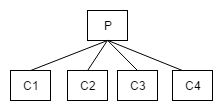
\includegraphics[width=0.5\linewidth]{figure/treecp}
	\caption[A sub tree with parent and children node]{A sub tree with parent and children node}
	\label{fig:treecp}
\end{figure}

\begin{figure}[H]
	\centering
	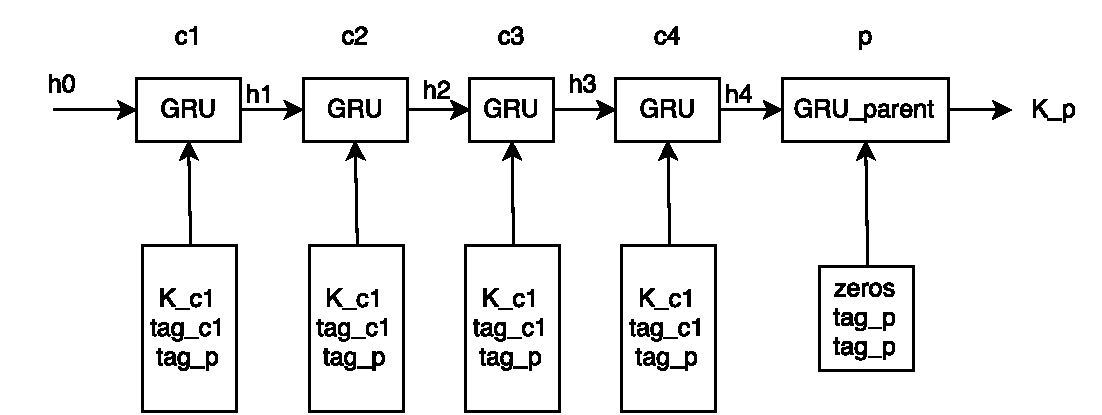
\includegraphics[width=0.7\linewidth]{figure/cvtgru}
	\caption[Constituency VT Tree-GRU]{Constituency VT Tree-GRU}
	\label{fig:cvtgru}
\end{figure}

\begin{figure}[H]
	\centering
	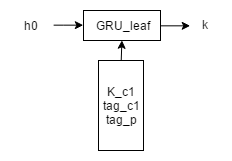
\includegraphics[width=0.4\linewidth]{figure/gruleaf}
	\caption[Constituency VT Tree-GRU leaf case]{Constituency VT Tree-GRU leaf case}
	\label{fig:gruleaf}
\end{figure}

\subsubsection{Dependency}
Each sentences are in Dependency Parse Tree using CoreNLP. For each node in parse tree, we also annotate POS-tag (Part-of-speech tag) and Universal Dependencies (rel).
We build a model similar to constituency case, with a chain GRU for each sub tree. However, we does not put parent node at the end of the chain. Instead, parent node and child node are sorted according to their position in sentences. We take node state k, node POS-tag, node dependency relationship type vs head word as input for GRU timestep. At parent node, we set dependency relationship type is 'self' and node states k set to zeros vector. We take hidden state of last timestep as node state k for parent node. In case of leaf node, we treat it as parent node without children. We build GRU chain with only parent node for leaf case. Fig \ref{fig:dependencyvtgru} illustrate Dependency VT GRU model.

\begin{figure}[h]
	\centering
	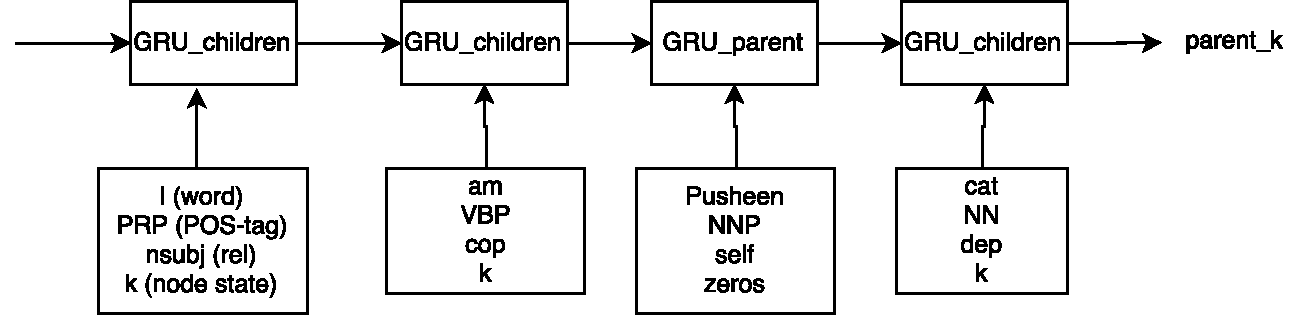
\includegraphics[width=0.5\linewidth]{figure/dependencyvtgru}
	\caption[Dependency VT GRU]{Dependency VT GRU}
	\label{fig:dependencyvtgru}
\end{figure}

\subsubsection{Training method and hyper-parameter}

\subsection{CNN-TreeLSTM}\label{sec:CNNtree}
\subsubsection{Training method and hyper-parameter}


\section{Improving continuous distributed word presentation}

\subsection{Training Glove embedding on Amazon reviews data set}

\subsection{Using hierarchical CNN to improve Glove embedding}

\subsubsection{Training method and hyper-parameter}


\section{Combining better sentence composition and distributed word presentation}

\subsubsection{Training method and hyper-parameter}
